\documentclass{beamer}
\usepackage{./presentation_style}
\mode<presentation>{
    \usetheme{Madrid}
%    \usetheme{Pittsburgh}
%    \usetheme{metropolis}
}





% To remove the footer line in all slides 
\setbeamertemplate{footline}

% To replace the footer line in all slides with a simple slide count 
\setbeamertemplate{footline}[page number]

% To remove the navigation symbols from the bottom of all slides 
\setbeamertemplate{navigation symbols}{} 


%\setbeamersize{text margin left=5mm,text margin right=5mm} 
%\addtobeamertemplate{frametitle}{}{\vspace{-3em}} % decrease




% ---------- Title Page ----------------
 % The short title appears at the bottom of every slide, the full title is only on the title page
\title{Microlocal Analysis \\ 
    \large with Applications to Non-Elliptic Fredholm Problems}

\author{Edmund Lau \\
Supervised by: Dr Jesse Gell-Redman} 

% Your institution as it will appear on the bottom of every slide, may be shorthand to save space
\institute[Unimelb] {
    The University of Melbourne \\ % institution for the title page
    \medskip
    \textit{elau1@student.unimelb.edu.au} % email address
}

\date{19 October 2018} 

\begin{document}
    
% ------------------------------------------ Title Frame 
\begin{frame}
\titlepage 
\end{frame}






%######################################### Section: Introduction
\section{Introduction} 
%------------------------- Frame : Introduction 1
\begin{frame}{Introduction}
A linear partial differential operator in $\R^n$ : 
\begin{equation}
P = P(x, D_x) = \sum_{\abs{\alpha} \leq k} c_\alpha(x) D^\alpha_x 
\end{equation}
\onslide<2->
where 
\begin{align*}
\alpha &= (\alpha_1, \alpha_2, \dots, \alpha_n) \in \N^n \tag*{ multi-index } \\
\abs{\alpha} &= \alpha_1 + \alpha_2 + \dots + \alpha_n \tag*{order of multi-index} \\
c_\alpha &\in C^\infty_\infty(\R^n) \tag*{ bounded  smooth functions} \\
D_{x_i} &= -i \p_{x_i} \\
D_x^\alpha & = \brac{-i \p_{x_1}}^{\alpha_1}\brac{-i \p_{x_2}}^{\alpha_2} \dots \brac{-i \p_{x_n}}^{\alpha_n} 
\end{align*}
\onslide<3->
Examples: 
\begin{align*}
&\Delta = - \p_{x_1}^2  - \dots - \p_{x_n}^2  \tag*{Laplace operator} \\
&\Box u = \p_{t}^2  - \p_{x_1}^2  - \dots - \p_{x_n}^2 \tag*{Wave operator} 
\end{align*}
\end{frame} 
% ------------------------- End Frame 


%------------------------- Frame : Introduction 2
\begin{frame}{Introduction}
An order $k \in \N$ linear partial differential equation (PDE) : 

\begin{equation*}
P u = f, \quad u, f \in \sch'(\R^n)
\end{equation*}

%\onslide<1->
%Smooth solution and forcing: 
%\begin{align*}
%C^\infty(\R^n) \ni u, \, f : \R^n \to \C 
%\end{align*}

\onslide<2-> 
Weak solution and forcing: 
\begin{align*}
u : \sch(\R^n) & \to \C \\
\varphi &\mapsto u(\varphi)
\end{align*}
\begin{align*}
\varphi  \in \sch(\R^n)  \iff 
 \varphi \in C^\infty \text{ and }  \sup_{x} \abs{x^\beta D^\alpha_x \varphi (x)} < \infty 
\end{align*}

\end{frame} 
% ------------------------- End Frame 


%------------------------- Frame : Introduction 3
\begin{frame}{Introduction}
%Given a PDE, $P u = f$, the all important questions are 
\begin{description}
    \item[Existence]<1-> For which $f$ can we some solution $u$? 
    \item[Uniqueness ]<2->  If that's possible,  is it the only one? 
    \item[Regularity ]<3-> How does the regularity of $f$ affect regularity of $u$? \\
    E.g. Does smooth begets smooth? 
\end{description}

\onslide<4> \textbf{Fredholm} theory tackles all three simultaneously! 

\end{frame} 
% ------------------------- End Frame 



% ------------------------------------------ Content Overview 
\begin{frame}{Overview}
\tableofcontents
\end{frame}

%######################################### Section: Fredholm operators
\section{Fredholm Operators and Regularity} 


%------------------------- Frame : Fredholm 1 
\begin{frame}{Fredholm Operators}
\begin{definition}[Fredholm operators]
    A continuous linear operator $T : \X \to\Y$ between Banach spaces $\X$ and $\Y$ is Fredholm, if 
    \begin{itemize}
        \item $T$ has closed range, i.e. $T(\X)$ is closed in $\Y$, 
        \item $\ker(T) \subset \X $ is finite dimensional, 
        \item $\coker(T) := \Y / T(\X)$ is finite dimensional. 
    \end{itemize}
\end{definition}
\pause
Suppose $Tx = y$ for a given $y \in \Y$. 
\begin{description}
    \item[Existence] a solution $x \in \X$ exist if and only if  $y \in \coker(T)^\perp $. 
    \item[Uniqueness] the solution is unique if and only if $\ker(T) = 0$. 
\end{description}
\pause
$T$ Fredholm \\
$\leadsto$ existence and uniqueness reduce to finite dimensional linear algebra. 

\end{frame}

%------------------------- Frame : Fredholm estimates
\begin{frame}{Fredholm Estimate}
In PDE, we would like  topological / algebraic statements $\leadsto$ estimates. 
\pause
\begin{theorem}[Fredholm Estimate] \label{theorem: fredholm estimates}
    Let $\X$, $\Y$, $\mathcal{Z}$ be Banach spaces.  If 
    \begin{itemize}
        \item $T : \X \to \Y$ is continuous, 
        \item $\X$ is compactly contained in $\mathcal{Z}$, i.e.  $\iota : \X\hookrightarrow \mathcal{Z}$ is compact, 
        \item for all $x \in \X$, there exist $C > 0$ such that the  following estimate hold
        \begin{align}
        \norm[x]_\X \leq C \brac{\norm[Tx]_\Y + \norm[x]_\mathcal{Z}}
        \end{align}
    \end{itemize}
    then $T$ is \textit{semi-Fredholm}
    \begin{itemize}
        \item the image, $T(\X)$ is closed, and
        \item $T$ has finite dimensional kernel. 
    \end{itemize} 
\end{theorem}


\end{frame} 
% ------------------------- End Frame 

%------------------------- Frame : Fredholm problem 
\begin{frame}{Constructing a \textit{Fredholm problem}} 
What's a Fredholm differential operator? $\dots $ what's $\X$ and $\Y$? 
\begin{block}{Fredholm Problem}
    Given a differential operator $P$, can we construct solution spaces $\X$ and $ \Y$,  so that $$P : \X \to \Y$$ is Fredholm? 
\end{block}
\pause 

What's the link to \textit{regularity}? Sobolev Space! 

\end{frame} 
% ------------------------- End Frame 

%------------------------- Frame : Sobolev space
\begin{frame}{Sobolev Space}
\begin{definition}
    The Sobolev space of order $k \in \N$ on $\R^n$,  $H^k(\R^n) \subset \sch'(\R^n)$  is defined by 
    \begin{align*}
    u \in H^k(\R^n) 
    &\iff D^\alpha u \in L^2(\R^n) \text{ whenever } \abs{\alpha} \leq k\\
    &\iff \sym[\xi]^k \widehat{u}(\xi) \in L^2(\R^n). 
    \end{align*}
\end{definition}

\begin{align*}
\sym[\xi] &:= \brac{1 + \abs{\xi}^2}^{1/2} = \brac{1 + \abs{\xi_1}^2+ \dots + \abs{\xi_n}^2}^{1/2} \\
\widehat{u}(\xi) &:= \F u(\xi)  = \frac{1}{(2\pi)^{n/2}} \int e^{-ix \cdot \xi} u(x)\d[x] 
\end{align*}

Hilbert space structure that keeps track of (global) regularity data of $u$. 
\begin{align*}
    \norm[u]_{H^k} = \underbrace{\norm[u]_{L^2}}_{\text{ global decay}}  + \underbrace{\sum_{\abs{\alpha} \leq k} \norm[D^\alpha u ]_{L^2} }_{\text{ $k$ times differentiable}} 
\end{align*}

\end{frame} 


%------------------------- Frame : Sobolev space generalisation 
\begin{frame}{Sobolev Space on Closed Manifold}
Let $M$ be a smooth closed $n$-manifold (compact without boundary), $s \in \R$, $u \in \brac{C^\infty(M)}'$, then 
\begin{align*}
u \in H^s(M) \iff \brac{\chi \cdot  u} \circ \Phi^{-1} \in H^s(U)
\end{align*} 
for any chart $\Phi : \widetilde{U} \to U \subset \R^n$ and smooth bump function $\chi \in C^\infty(M)$ compactly supported in the chart domain $\widetilde{U}$. \\[3em]
\pause 
Henceforth, $M$ is either $\R^n$ or a closed $n$-manifold. 
\end{frame} 
% ------------------------- End Frame 

%------------------------- Frame : General strategy
\begin{frame}{General Strategy}
%Given differential operator $P$ on manifold $M$: 
Existence, uniqueness, regularity $\leadsto$ 
\begin{block}{} 
     For what $s, s' \in \R$ can we prove 
     \begin{align*}
     \norm[u]_{H^s} \leq C \brac{\norm[Pu]_{H^{s'}} + \norm[u]_{H^{N}}}. 
     \end{align*}  
     so that $P: H^s(M) \to H^{s'}(M)$ is (semi-) Fredholm? 
\end{block}

For \textbf{elliptic operators}: 
\begin{center}
    any $s$ and $s' = s - m$. 
\end{center}
For \textbf{non-elliptic operators}: 
\begin{center}
    any $s$ and $s' = s - m + 1$. \\
    Only certain subsets of Sobolev spaces allowed. 
\end{center}

\end{frame} 
% ------------------------- End Frame 


%######################################### Section: Elliptic case
\section{``Elliptic operators are Fredholm"} 
%------------------------- Frame : Elliptic regularity
\begin{frame}{``Elliptic operators are Fredholm"} 
How do we get such an estimate? 

% ------------------------- End Frame 
\begin{theorem}[Elliptic regularity]
    Let $P$ be an order $m \in \R$ \textcolor<2->{red}{\only<2->{\LARGE} elliptic}
%     \only<2->{\textcolor<2->{red}{\Large (pseudo-)}} 
    differential operator on an $n$-manifold, $M$. Suppose we know \textit{a priori} that $u \in H^{N}(M)$ for some $N \in \R$. Then, for any $s \in \R$
    \begin{align*}
    (f = ) Pu \in H^{s}(M) \implies u \in H^{s + m}(M)
    \end{align*}
    and $u$ satisfies the estimates: $\exists C > 0$
    \begin{align*}
    \norm[u]_{H^{s + m}} \leq C \brac{\norm[Pu]_{H^s} + \norm[u]_{H^N}}. 
    \end{align*}
\end{theorem}

\end{frame} 


%------------------------- Frame : Elliptic operator
\begin{frame}{Elliptic operator}
Elliptic operators generalise the Laplace operator: $\Delta \uncover<2->{+1}$. \\
\onslide<3-> 
Fourier transform + integration by parts $\implies$ $\F D_x = \xi \F $ 
\begin{align*}
\brac{\Delta + 1} u(x) = \F^{-1} \F (\Delta + 1) u = \F^{-1} (1 + \abs{\xi}^2) \F u 
%\frac{1}{(2\pi)^n} \int e^{i(x - y) \cdot \xi} \brac{1 + \abs{\xi}^2} u(y) \d[y]  \d[\xi]
\end{align*}
\onslide<4-> 
We expect an inverse $\dots$ 
\begin{align*}
\brac{\Delta + 1}^{-1} \brac{\Delta + 1} u(x) = \F^{-1} (1 + \abs{\xi}^2)^{-1} (1 + \abs{\xi}^2) \F u = u 
%&= \frac{1}{(2\pi)^n} \int e^{i(x - y) \cdot \xi} \underbrace{\brac{1 + \abs{\xi}^2}^{-1} \brac{1 + \abs{\xi}^2}}_{= 1} u(y) \d[y]  \d[\xi] = u(x) 
\end{align*}
$\brac{1 + \abs{\xi}^2}^{\pm 1} $ are examples of \textbf{symbols}! 
\end{frame} 

%------------------------- Frame : Pseudodifferential operator
\begin{frame}{Pseudodifferential operator}
Question: What is $\brac{\Delta + 1}^{-1}$? Answer: \textbf{pseudo}differential operator. 
\begin{align}
P(x, D_x) u = \frac{1}{(2\pi)^n} \int e^{i(x - y) \cdot \xi} p(x, \xi) u(y) \d[y] \d[\xi]  \label{eq: action of symbol} 
\end{align}
\onslide<2-> 
\begin{definition} A smooth function $p(x, \xi) \in C^\infty(\R^{n}; \R^n)$ is a symbol of order $m \in \R$, i.e. $p \in S^{m}_\infty(\R^{n}; \R^n)$, if
    \begin{align*}
    \abs{D^{\alpha}_x D^\beta_\xi p(x, \xi)} \leq C_{\alpha, \beta, \gamma}  \sym[\xi]^{m - \abs{\beta}}, \quad C_{\alpha, \beta}  > 0
    \end{align*}
    for any multi-index $\alpha, \beta \in \N^n$. \\
    
    A pseudodifferential operator, $P \in \Psi^{m}_{\infty}(\R^n)$ of order $m$ with (left reduced) symbol $p \in S^{m}_\infty(\R^{n}; \R^n)$ has action on $u \in \sch'(\R^n)$ given by (\ref{eq: action of symbol}). 
\end{definition}
\end{frame} 

%------------------------- Frame : Prove of elliptic regularity
\begin{frame}{Pseudodifferential operators}
\begin{lemma}
    %The total spaces $\cup_{m} S^{m}_\infty(\R^{n}; \R^n)$ and $\cup_{m} \Psi^{m}_{\infty}(\R^n)$ form filtered *-algebra over $\C$. 
    If $P \in \Psi^{m}_{\infty}(M)$ for some $m \in \R$, 
    \begin{enumerate}
        \item $P : H^{s}(M) \to H^{s - m}(M)$ is continuous for any $s \in \R$. 
        \item If $P$ is \textbf{elliptic} of order $m$, i.e. its symbol $p$ satisfies
        \begin{align*}
        \abs{p(x, \xi)} \geq \epsilon \sym[\xi]^m \tag*{ in $\abs{\xi} > \epsilon$ for some $\epsilon > 0$ } 
        \end{align*}
        then there exist \textit{parametrix} $Q \in \Psi^{-m}_{\infty}(M)$ such that 
        $$QP - 1: H^{s}(M) \to H^{s'}(M)$$
         is continuous for any $s, s' \in \R$. 
    \end{enumerate}
\end{lemma}
\end{frame} 

% ------------------------------ Frame: Proof elliptic regularity 
\begin{frame}{Proof of Elliptic Regularity}
$P$ elliptic with parametrix $Q$. Given $u \in H^N(M)$. 
\onslide<1->Given any $u \in H^N(M)$. Write $u = QP u -  \brac{QP - 1} u$. 
\onslide<2->
\begin{align*}
\norm[u]_{H^{s + m}} 
&\leq \underbrace{\norm[QPu]_{H^{s + m}}}_{\leq C \norm[Pu]_{H^s}} + \underbrace{\norm[\brac{QP - 1}u]_{H^{s +m}}}_{\leq C \norm[u]_{H^N}}
\end{align*}
using continuity $Q: H^{s +m} \to H^{s}$ and $(QP - 1): H^{s + m} \to H^{N}$.  \\
\onslide<3->
We get 
\begin{align*}
\norm[u]_{H^{s + m}} \leq C \norm[Pu]_{H^s} + C \norm[u]_{H^N}. 
\end{align*}
\end{frame} 
% ------------------------------ End Frame


%######################################### Section: Non-elliptic case
\section{A Non-elliptic Fredholm problem}

%------------------------- Frame : Non-Elliptic Fredholm Problem
\begin{frame}{Non-elliptic Fredholm problem}
Recent work by \cite{Vasy, Gell-Redman} show that we can construct Fredholm problem for \textbf{non-elliptic} operators too! \\
%We'll illustrate by sketching the proof for a pertubation of the  wave operator 
\begin{theorem}[Main theorem] 
    There exist a perturbation $Q$ of the wave operator $\Box$ on $\T^{1 + n}$ and a subspace $\X^{s + 2} \subset H^{s+ 2}(\T^{1 +n})$ for each $s \in \R$, such that the operator: 
    \begin{align*}
    (\Box - iQ): \mathcal{X}^{s + 2} \to H^{s + 1}(\T^n)
    \end{align*}
    is Fredholm. 
\end{theorem}
\begin{align*}
\T^{1 + n} &:= \S^1_t \times  \underbrace{\S^1_{x_1} \times \S^1_{x_2} \times \dots \times \S^1_{x_n}}_{n} \\
\Box &:= \p_t^2 - \sum_{j = 1}^{n -1} \p_{x_j}^2, \quad p(t, x, \tau, \xi) = \abs{\xi}^2 - \tau^2
\end{align*}
\end{frame} 
% ------------------------- End Frame 

%------------------------- Frame : Microlocalisation
\begin{frame}{Microlocal Viewpoint}
\only<1>{
Global ellipticity \\
$\iff$ $\abs{p(t, x, \tau, \xi)} \geq \epsilon \sym[(\tau, \xi)]^2$ whenever $ \abs{(\tau, \xi)} > 1/\epsilon$.\\
} 
\only<2->{
Microlocal ellipticity at a point $(t_0, x_0, \tau_0, \xi_0) \in T^*\T^{1 + n} \setminus 0$ \\
$\iff$ $\abs{p(t, x, \tau, \xi)} \geq \epsilon \sym[(\tau, \xi)]^2$ in }
\onslide<3->
\begin{center}
    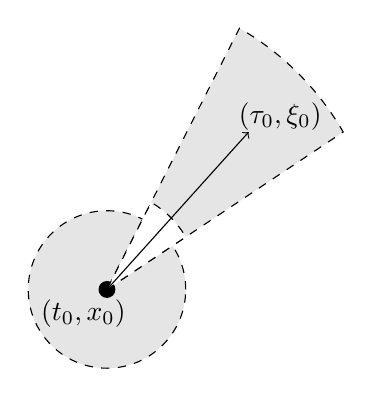
\begin{tikzpicture}
    \draw [fill=gray!20!white, dashed] (0, 0) circle [radius=1]; 
    \draw [fill=black] (0, 0) circle [radius=0.1]; \node at (-0.3, -0.3) {$(t_0, x_0)$}; 
    
    \filldraw[fill=gray!20!white, dashed]
    (0,0) -- (3, 2) arc (30:60:3.6) -- (0,0);
    
    \filldraw[fill=white!20!white, dashed]
    (0,0) -- (1, 0.66666) arc (30:60:1.2) -- (0,0);
    
    \draw [-> ] (0, 0) -- (1.8, 2); \node at (2.2, 2.2) {$(\tau_0, \xi_0)$};
    \end{tikzpicture}
\end{center}
\onslide<4->
$\Ell^2=  \set{\text{points in phase space where $p$ is elliptic}} \setminus 0 $ \\
$\Char^2 = \Ell^m(\Box)^c \setminus 0$. 

Note: For differential operators: Elliptic $\iff$  principal symbol is non-zero (outside of zero section). 
\end{frame} 
% ------------------------- End Frame 

%------------------------- Frame : Ingredients
\begin{frame}{Two Major Ingredients}
\begin{theorem}[Microlocal elliptic regularity]
        Let $P \in \Psi^{m}_{\infty}(\R^n)$ and $u \in \sch'(\R^n)$. If for some $\chi_2 \in \Psi^{0}_{\infty}(\R^n)$, $\chi_2 Pu \in H^{s}(\R^n)$, then for any other $\chi_1 \in \Psi^{0}_{\infty}(\R^n)$ such that $\WF'(\chi_1) \subset \Ell^m(P) \cap \Ell^0(\chi_2)$ we have $\chi_1 u \in H^{s + m}(\R^n)$ and it satisfies the estimate: $\forall N \in \R$, $\exists C > 0$ 
        \begin{align*}
        \norm[\chi_1 u]_{H^{s +m}} \leq C \brac{\norm[\chi_2 Pu]_{H^s} + \norm[u]_{H^N}}. 
        \end{align*}
\end{theorem}
\begin{center}
    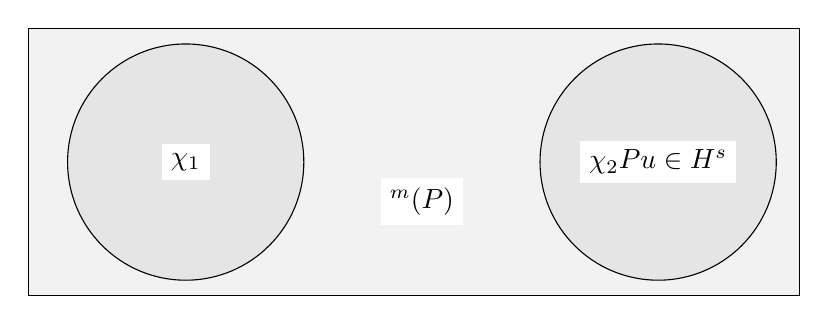
\begin{tikzpicture}
    \draw [fill=gray!10!white] (-5, -0.2) rectangle (4.8, 3.2); 
    \node [fill=white, dashed] at (0, 1) {$\Ell^m(P)$};  
    
    \draw [fill=gray!20!white] (-3, 1.5) circle [radius=1.5]; \node [fill=white] at (-3, 1.5) {$\supp \chi_1$}; 
    
    \draw [fill=gray!20!white] (3, 1.5) circle [radius=1.5]; \node [fill=white] at (3, 1.5) {$\chi_2 Pu \in H^s$}; 
    

    \end{tikzpicture}
\end{center}
\end{frame} 
% ------------------------- End Frame 


% ------------------------------ Frame
\begin{frame}{Two Major Ingredients}
\begin{theorem}[Propagation of singularities] \label{theorem: propagation of singularity estimates}
    Let $P \in \Psi^{m}_{\infty}(\R^n)$ is a properly supported pseudodifferential operator with polyhomogeneous principal $\sigma_m(P) = p - iq$ with real $p, q$. If we have $\chi_1, \chi_2, \chi_3 \in \Psi^{0}_{\infty}(\R^n)$ and $q \geq 0$ on $\WF'(\chi_3)$ and every $(x, \xi) \in WF'(P)$ is in the integral curve of $H_p$ originating from $\Ell^0(\chi_2)$, then for all $s, N \in \R$ and $u \in C^\infty(\R^n)$, there exist $C > 0$ such that 
    \begin{align*}
    \norm[\chi_1 u]_{H^{s + m}} \leq C\brac{\norm[\chi_2 u]_{H^s} + \norm[\chi_3 Pu]_{H^{s + 1}} + \norm[u]_{H^{N}}}. 
    \end{align*}
\end{theorem}
\begin{center}
    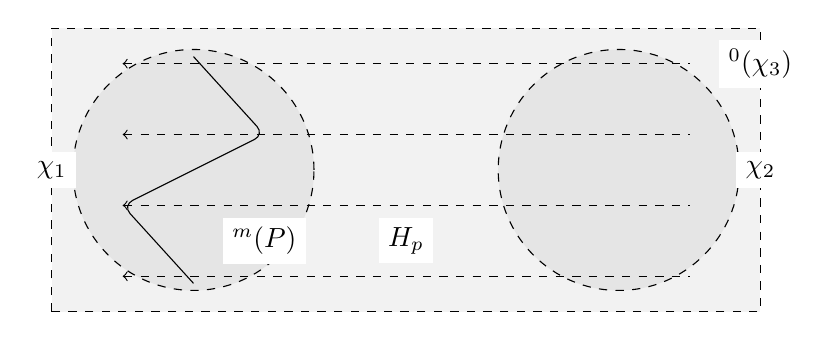
\begin{tikzpicture}[scale=0.9]
    \draw [fill=gray!10!white, dashed] (-5, -0.5) rectangle (5, 3.5); 
    \node [fill=white] at (5, 3) {$\Ell^0(\chi_3)$}; 
    
    \draw [fill=gray!20!white, dashed] (-3, 1.5) circle [radius=1.7]; 
    \node [fill=white] at (-5, 1.5) {$\supp \chi_1$}; 
    
    \draw [fill=gray!20!white, dashed] (3, 1.5) circle [radius=1.7]; 
    \node [fill=white] at (5, 1.5) {$\supp \chi_2$}; 
    
    \draw [<-, dashed] (-4, 0) -- (4, 0); 
    \draw [<-, dashed] (-4, 1) -- (4, 1); 
    \draw [<-, dashed] (-4, 2) -- (4, 2); 
    \draw [<-, dashed] (-4, 3) -- (4, 3); 
    \node [fill=white] at (0, 0.5) {$H_p$}; 
    
    \draw [rounded corners] (-3, -0.1) -- (-4, 1) -- (-2, 2) -- (-3, 3.1); 
    \node [fill=white] at (-2, 0.5) {$\Char^m(P)$}; 
    \end{tikzpicture}
\end{center}
\end{frame} 
% ------------------------------ End Frame


%%------------------------- Frame : Reminder of reduced goal
%\begin{frame}{Current Goal}
%Main idea : Introduce an elliptic region from which to propagate! Perturbation $Q = \chi(t) \p_t^2$. 
%\begin{align*}
%Q &= \chi(t) \p_t^2 \\
%\X^s &= \set{u \in H^{s} \wh \brac{\Box - iQ} u \in H^{s -1}} \subset H^s(\T^{1 + n}) 
%\end{align*}
%For semi-Fredholm, we want
%\begin{align*}
%\underbrace{\norm[u]_{H^s} + \norm[(\Box - iQ)u]_{H^{s-1}}}_{ = \norm[u]_{\X^s}}  \leq C \brac{\norm[(\Box - iQ)u]_{H^{s-1}} + \norm[u]_{H^N}} \\
%\end{align*}
%\begin{block}{Target estimate}
%    For all $s, N \in \R$, there exist $C > 0$ : 
%    $$\norm[u]_{H^s}  \leq C \brac{\norm[(\Box - iQ)u]_{H^{s-1}} + \norm[u]_{H^N}}$$
%\end{block}
%\end{frame} 
%% ------------------------- End Frame 

%------------------------- Frame : 
\begin{frame}{Constructions}
Main idea : Create enough elliptic region! $\Box - iQ = \Box - i \chi(t) \p_t^2$. 

\begin{center}
    \begin{tikzpicture}[scale=0.8]
    \draw [] (0, 0) rectangle (8, 8);
    \node at (8.3, -0.1) {$x$};
    \node at (-0.1, 8.3) {$t$}; 
    \node at (-0.2, -0.2) {$0$}; 
    \pause 
    
    \draw[pattern=north west lines, pattern color=blue, opacity=0.5] (0, 0) rectangle (8, 2);
    \draw[pattern=north west lines, pattern color=blue, opacity=0.5] (0, 6) rectangle (8, 8);
    \node at (8.6, 6) {$1 - \delta$};
    \node at (8.6, 2) {$\delta$};
    \node [fill=white]  at (4, 7) {$U_1 :=  \set{\chi(t) \equiv 1}$ };
    \pause 
    
    \draw [->, thick] (-0.5, 0) -- (-3, 0); 
    \draw [->, thick] (-0.5, 0) -- (-0.5, 8);
    \draw [-, thick] (-2.5, 0.1) -- (-2.5, -0.1);
    \node at (-3.3, -0.3) {$\chi(t)$};
    \node at (-2.5, -0.3) {1}; 
    
    \draw (-2.5, 0) -- (-2.5, 2);5
    \draw[rounded corners=8pt] (-2.5, 2) -- (-2.5, 2.24) -- (-1, 2.25) -- (-0.5, 2.5);
    \node at (-2.5, 8) (right start) {};
    
    \draw (-2.5, 8) -- (-2.5, 8 - 2);
    \draw[rounded corners=8pt] (-2.5, 8 - 2) -- (-2.5, 8 - 2.24) -- (-1, 8 - 2.25) -- (-0.5, 8 - 2.5);
    
    \draw  [dashed] (-2.5, 2) -- (8.1, 2);
    \draw  [dashed] (-2.5, 6) -- (8.1, 6);
    \draw  [dashed] (-0.5, 5.5) -- (8.1, 5.5);
    \draw  [dashed] (-0.5, 2.5) -- (8.1, 2.5);
    \pause 
    
    \draw[pattern=north east lines, pattern color=red, opacity=0.5] (0, 2.5) rectangle (8, 5.5); 
    \node [fill=white]at (4, 4) {$\abs{\xi}^2 - \tau^2 $}; 
    \node [fill=white] at (4, 1) {$\abs{\xi}^2 - \tau^2 + i \tau^2$};
    \end{tikzpicture}
\end{center}
\end{frame} 
% ------------------------- End Frame 


%------------------------- Frame : 
\begin{frame}{Hamilton flow of $\sigma_2(\Box)$ }
Hamiltonian flow: $\exp(sH_ p)(t, x, \tau, \xi) = (t + s\tau, x + s \xi, \tau, \xi)$

\begin{center}
    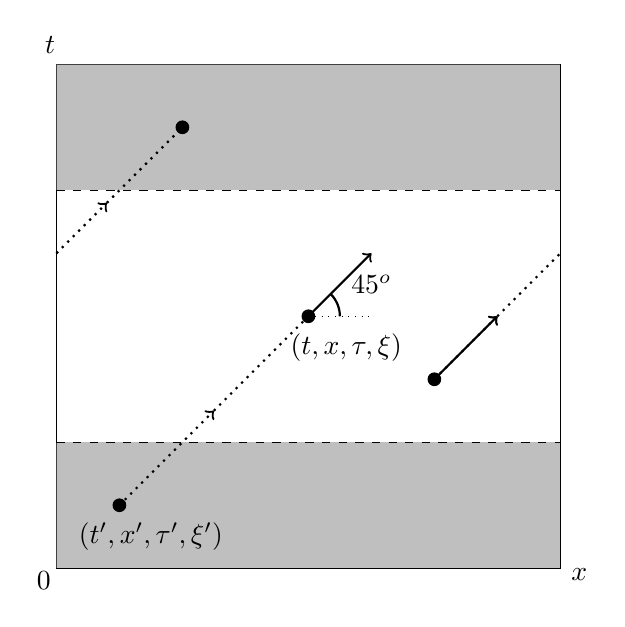
\begin{tikzpicture}[scale=0.8]
    \draw [] (0, 0) rectangle (8, 8);
    \fill [gray, opacity=0.5] (0, 0) rectangle (8, 2);
    \fill [gray, opacity=0.5] (0, 6) rectangle (8, 8);
    \draw [dashed] (0, 2) -- (8, 2);
    \draw [dashed] (0, 6) -- (8, 6);
    
    \draw [fill=black] (4, 4) circle [radius = 0.1]; 
    \draw [->, thick] (4, 4) -- (5, 5);
    \node at (4.6, 3.5) {$(t, x, \tau, \xi)$}; 
    
    
    \draw [fill=black] (1, 1) circle [radius = 0.1]; 
    \draw [->, thick, dotted] (1, 1) -- (2.5, 2.5);
    \draw [thick, dotted] (2.5, 2.5) --  (4, 4); 
    \node at (1.5, 0.5) {$(t', x', \tau', \xi')$}; 
    
    
    \draw [dotted] (4, 4) -- (5, 4);
    \draw [thick] (4.5, 4) arc (0:45:0.5); 
    \node at (5, 4.5) {$45^o$}; 
    
    \node at (8.3, -0.1) {$x$};
    \node at (-0.1, 8.3) {$t$}; 
    \node at (-0.2, -0.2) {$0$};
    
    
    
    \draw [fill=black] (6, 3) circle [radius = 0.1]; 
    \draw [->, thick] (6, 3) -- (7, 4);
    \draw [->, thick, dotted] (6, 3) -- (7, 4);
    \draw [thick, dotted] (7, 4) -- (8, 5);
    \draw [->, thick, dotted] (0, 5) -- (0.8, 5.8); 
    \draw [thick, dotted] (0.8, 5.8) -- (2, 7); 
    \draw [fill=black] (2, 7) circle [radius = 0.1];
    \end{tikzpicture}
\end{center}
\end{frame} 

% ------------------------- End Frame 


%------------------------- Frame : 
\begin{frame}{Constructions}

\begin{itemize}
    \item (principal) symbol of the form $p - iq$, $p = \sigma_2(\Box)$, $q \geq 0$. (\checkmark)
    \item Elliptic region that propagates to hit every point in $\Char^2(\Box - iQ)$. (\checkmark)
\end{itemize}
\onslide<2->
Propagation of singularity $\implies$

\begin{align*}
    \norm[\chi_1 u]_{H^{s + m}} &\leq C \norm[\chi_2 u]_{H^s} + C\norm[\chi_3 Pu]_{H^{s + 1}} + \norm[u]_{H^{N}} \\
    \onslide<3->{\norm[u]_{H^{s + 2}} &\leq C \underbrace{\norm[\chi(t) u]_{H^s}}_{\text{elliptic region!}} + C\norm[(\Box - iQ) u]_{H^{s + 1}} + C \norm[u]_{H^{N}}}\\
    \onslide<4->{\norm[u]_{H^{s + 2}} &\leq C' \norm[\Box - iQ]_{H^{s -2}} + C\norm[(\Box - iQ) u]_{H^{s + 1}} + C' \norm[u]_{H^{N}}}\\
    \onslide<5->{\norm[u]_{H^{s + 2}} &\leq C'' \brac{\norm[(\Box - iQ) u]_{H^{s + 1}} + \norm[u]_{H^{N}}}}\\
\end{align*}
\end{frame}
% ------------------------- End Frame 

% ------------------------------ Frame
\begin{frame}{}
Almost there! 
\begin{align*}
\norm[u]_{H^{s + 2}} &\leq C'' \brac{\norm[(\Box - iQ) u]_{H^{s + 1}} + \norm[u]_{H^{N}}}
\end{align*}
Which suggest the Hilbert space domain that we want is 
\begin{align*}
\X^s = \set{u \in H^{s + 2} \wh (\Box - iQ) u \in H^{s + }}. 
\end{align*}
And
\begin{align*}
\Box - iQ : \X^s \to H^{s + 1}
\end{align*}
is (semi-) Fredholm for any $s \in \R$. 
\end{frame} 
% ------------------------------ End Frame



%------------------------- Frame : THE END
\begin{frame}{The End}
\begin{center}
    \LARGE Thank you! \\[3em]
    Questions are welcomed! 
\end{center}
\end{frame} 
% ------------------------- End Frame 


\end{document}

%% ------------------------------------------ Sandbox frame
%\appendix
%\section*{sandbox}
%
%Fourier analysis relates the (global) regularity of functions to their fourier transform. e.g. in the 'superposition of wave' picture, only waves with high frequency can approximate jump discontinuity, linking continuity with the decay of fourier coefficients. 
%Microlocal analysis also keeps track of the direction of decay. 
%\begin{theorem}[Rank-nullity]
%    If $T : V \to W$ be a linear operator between finite dimensional vector space $V$ and $W$, then 
%    \begin{align*}
%    \mathrm{Ind}(T) := \dim \ker T - \dim \coker T = \dim W - \dim V. 
%    \end{align*}
%\end{theorem}
%\begin{theorem}[Atiyah-Singer index theorem]
%    Given
%    \begin{itemize}
%        \item $X$ a smooth comapct manifold, 
%        \item $E, F$ smooth vector bundles over $X$, 
%        \item $P : \Gamma(E) \to \Gamma(F)$ be an elliptic differential operators between the space of sections of $E$ and $F$. 
%    \end{itemize}
%    Then, $P$ is Fredholm and its Fredholm index is related to its topological index. 
%\end{theorem}
%
%
%


%\begin{frame}{Fredholm operators}
%\begin{align*}
%T x = y \quad x \in X, \, y \in Y
%\end{align*}
%\begin{itemize}
%    \item $\dim \coker(T) < \infty $ means that solutions exist if and only if 
%    $$\omega_1(y) = \omega_2(y) = \dots \omega_n(y) = 0$$ 
%    where $\set{\omega_i}_{i = 1}^n$ is any basis of $\coker(T)$. \todo{with isomorphism to the perpendicular space}
%    
%    \item $\dim \ker(T) < \infty$ means that solution is unique up to addition of element in a finite dimensional space. 
%    
%    \item $T$ is invertible modulo compact operators (limits of finite rank operators). 
%\end{itemize}
%
%\end{frame}


%\begin{frame}{Fredholm Index}
%\begin{definition}
%    The index of a Fredholm operator $T$ is defined by
%    \begin{align*}
%    \ind(T) := \dim \ker(T) - \dim \coker(T). 
%    \end{align*}
%\end{definition}
%\begin{itemize}
%    \item $\ind : \mathrm{Fred}(X, Y) \to \Z$ is a continuous map. 
%    \item Unlike kernel and cokernel themselves, $\ind$ is well-behaved. \todo{example on the circle.}
%    \item \todo{something about Atiyah-Singer index which only works for elliptic diff on compact manifolds} 
%\end{itemize}
%
%
%\end{frame}
%
%
%
%\begin{frame}{Fredholm differential operators}
%\begin{theorem} \label{theorem: fredholm estimates}
%    Let $V$, $W$, $Y$ be Banach spaces, $T \in \L(V, W)$ and $K \in \K(V, Y)$. If for all $u \in V$, the estimate 
%    \begin{align*}
%    \norm[u]_V \leq C \brac{\norm[Tu]_W + \norm[Ku]_Y}
%    \end{align*}
%    holds for some positive real constant $C \in \R_{> 0}$, then the image, $T(V)$ is closed, and $T$ has finite dimensional kernel. 
%\end{theorem}
%
%Suppose we can show that the differential operator $P$ is Fredholm as a map 
%\begin{align*}
%P : H^{s} \to H^{s - m}
%\end{align*}
%
%\begin{align*}
%Pu = f \quad f \in H^s(M), u \in \sch'
%\end{align*}


% ------------------------- End Frame 

% ------------------------- End Frame 
% ------------------------- End Frame 
%\begin{frame}{``Ellitptic Operators are Fredholm"}
%\begin{example}[Laplacian]
%    $\Delta: H^{s} \to H^{s - 2}$
%    \begin{align*}
%    \norm[u]_{H^{s + 2}} \leq C \brac{\norm[\Delta u]_{H^s} + \norm[u]_{L^2}}. 
%    \end{align*}
%\end{example}
%
%\begin{proposition}
%    Let $A \in \Psi^{m}_{\infty}(\R^n)$ be elliptic and $u \in H^{N}(\R^n)$ for some $N \in \R$. Then, for any $s \in \R$
%    \begin{align*}
%    Au \in H^{s}(\R^n) \implies u \in H^{s + m}(\R^n)
%    \end{align*}
%    and $u$ satisfies the estimates: $\exists C > 0$
%    \begin{align*}
%    \norm[u]_{H^{s + m}} \leq C \brac{\norm[Au]_{H^s} + \norm[u]_{H^N}}. 
%    \end{align*}
%\end{proposition}
%
%
%\todo{
%    Elliptic regularity estimate. (compact and non-compact manifold case). 
%}
%
%\end{frame}

1
- Don't spend too much time on title page (introduce PDE) 

2
- Say too much about $D_x^\alpha$ (mixed partial derivative). 
- Move example of equation to example of operator on the first slide. 

3
- Take out lines about smooth solution and forcing
- "Here this equation make sense even weakly. " 
- Notation too confusing don't use $\ni$. 

4
- "For which $f$ can we find ...."
- "How does the regularity of $f$ influence the regularity of $u$." 


5: overview

6 
- Need to streamline where I define / discuss "Fredholm". 
- TYPO!!! $y \in \coker(T)^\perp$ 
- Don't say "finite number of conditions" 

7 
- "semi-fredholm" is a thing!!
- "control norm the norm of elements in the domain and a weaker norm" 


8
- Take out the answer! 


9 
- Practise! bound by 30 sec!!! 
- Keep it simple. 
- "Regularity space". 
- "Differentiable k-times" in $L^2$. 


10
- 4 sec
- "Generalising to closed manifold, ... locally ..." 


11
- Move compact containment to last line
- Just use $P: H^s \to H^{s'}$ remove $\X$ and $\Y$ . Answer for elliptic is yes, for non-elliptic we have to take subspace. 
- The point is that we reduce Fredholm estimate in the case of diff op to the following

12 
- "I know I owe you the definition of ellipticity" 
- Keep track of $\R^n$ and $M$!!! 

13
- Write $\F$ for the integral instead
- "Staring at that operator, it is clearly invertible"
- But wait? that's no longer a "differntial operator" 
- Say something quick about symbol: "They obey a bound that behaves that polynomial." 



- No more filtered algebra. 
- Define pseudo's on $M$ as well! 

- Change theorem to lemma (those concerning pseudo's) 
- After proof of elliptic reg, say something about closed manifold and fredholm!! 



Wave operator
- "We have seen that fredholm are important in PDE. Also seen that elliptic regularity in the form of estiamates give fredholmness". "Now the question is do we have estimates for non-elliptic ones" Yes, by recent work of \cite{}

- Change left hand side ot $s + m$ for uniformity. 




